\section{Concepts and Definitions}\label{sec:concepts}
%
All concepts, definitions, and algorithms discussed in this article
are illustrated on a commonly used dynamic system consisting of water
tanks that are connected with valves.
%
\subsection{Running Example}
%
The three-tank system is shown in figure~\ref{fig:three_tanks}. The
tanks are denoted as $T_1$, $T_2$, and $T_3$. They all have the same
area $A_1 = A_2 = A_3 = 3~[\textrm{m}^2]$. The three tanks are
indestructible and of infinite height representing an idealized
experiment.  We assume that $g = 10$ and the liquid is ``pure'' water
with density $\rho = 1$.
%
\begin{figure}[htb]
  \centering
  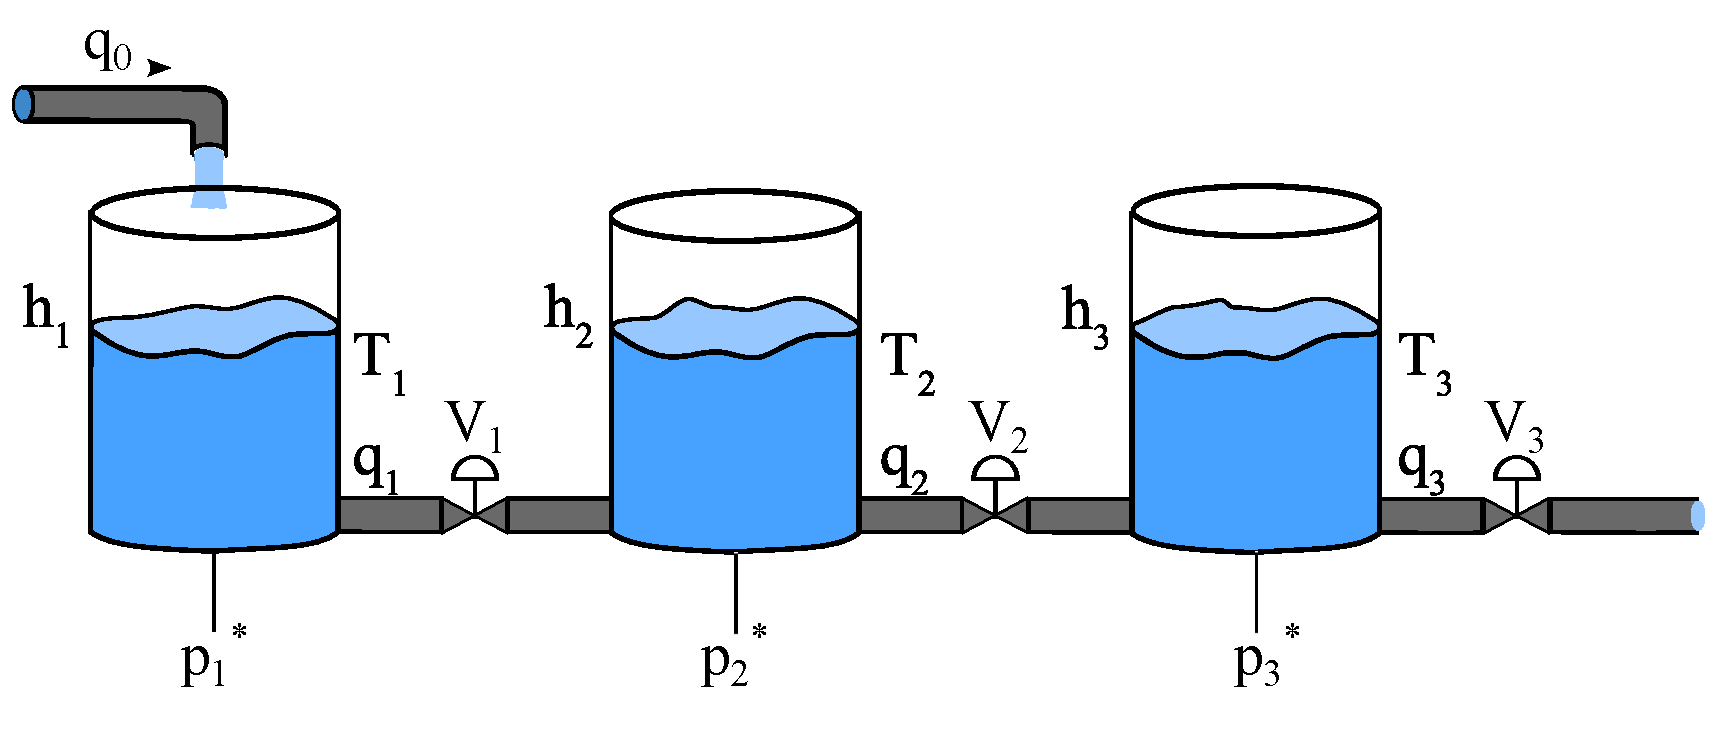
\includegraphics[width=1\columnwidth]{3-tanks}
  \caption{Diagram of the three-tank system.}
  \label{fig:three_tanks}
\end{figure}
\par\noindent
%
Tank $T_1$ is filled from a pipe $q_0$ with a constant flow of
$0.75~[\textrm{m}^3/\textrm{s}]$. It drains into $T_2$ via a pipe
$q_1$. The liquid level is denoted as $h_1$. There is a pressure
sensor $p_1$ connected to $T_1$ that measures the pressure in Pascals
[Pa]. Starting from Newton's (and Bernouli's) equations and
manipulating them (the actual derivation is irrelevant in this paper)
we derive the following Ordinary Differential Equation (ODE) that
gives the level of the liquid in $T_1$:
%
\begin{eqnarray}
%
\frac{d h_1}{dt} = \frac{q_0 - k_1 \sqrt{h_1 - h_2}}{A_1}\label{eq:ode1}
%
\end{eqnarray}
%
In eq.~\ref{eq:ode1}, the coefficient $k_1$ is the product of the
cross-sectional area of the tank $A_1$ and the area of the drainage
hole and $\sqrt{2g}$ and the friction/contraction factor of the
hole. We emphasize the use of $k_1$ because, later, we will be
``diagnosing'' our system in term of changes in $k_1$. Consider a
physical valve $R_1$ between $T_1$ and $T_2$ that constraints the flow
between the two tanks. We can say that the valve changes
proportionally to the cross-sectional drainage area of $q_1$ and hence
$k_1$. The diagnostic task is to compute the true value of $k_1$,
given $p_1$, and from $k_1$ we can compute the actual position of the
valve $R_1$.
%
The water levels of $T_2$ and $T_3$, denoted as $h_2$ and $h_3$
respectively, are given by:
%
\begin{eqnarray}\label{eq:tank1}
%
\frac{d h_i}{dt} = \frac{k_{i - 1} \sqrt{h_{i - 1} - h_i} - k_i \sqrt{h_i}}{A_i},
%
\end{eqnarray}
%
where $i$ is the tank index ($i \in \{2, 3\}$).
\par
Let us say that $k_1 = k_2 = k_3 = 0.75$.
\par
Finally, we turn the water level into pressure:
\begin{eqnarray}
p_i = \frac{g\,h_i\,A}{A} = g\,h_i\label{eq:pressure}
\end{eqnarray}
where $i$ is the tank index ($i \in \{1, 2, 3\}$).
\par
It is assumed that the initial water level in the three tanks is zero.
%
Let us continue with some notation and definitions.
%
\subsection{Compositional Modeling}
%
Consider a component library $\cl = \left\{C_1, C_2, \ldots,
C_n\right\}$ where each component $C_i$ for $i = \left\{1, 2, \ldots,
n\right\}$ is defined as \textit{a set} of models. Each set $C_i =
\left\{C_{i, 1}, C_{i, 2}, C_{i, 3}\right\}$ contains a non-linear,
linear, and qualitative model describing the behavior of the $C_i$
component.

We consider systems that can be described in terms of a set
${\vec{x}}(t)$ of state variables, $\vec{y}(t)$ of observable variables,
and $\vec{u}(t)$ of control variables.

\begin{definition}[Non-Linear Model]
We write the dynamic equations for a model in state-space form using
\begin{eqnarray}\label{eq:nonlinear}
\dot{\vec{x}}(t) & = & \psi (\vec{x}(t)) + \vec{u}(t))\\
\vec{y}(t) & = & \gamma (\vec{x}(t)), \vec{u}(t)),
\end{eqnarray}
where $\psi$ and $\gamma$ are non-linear functions.
\end{definition}
%
In the case of the three-tanks example, the non-linear model of $T_1$
is given by equations (\ref{eq:ode1}) and (\ref{eq:pressure}) and the
models of $T_2$ and $T_3$ are given by equations (\ref{eq:tank1}) and
(\ref{eq:pressure}).
%
\begin{definition}[Linear Model]
We write the linear dynamical equations for a model in state-space form using
\begin{eqnarray}\label{eq:linear}
\dot{\vec{x}}(t) & = & \mathbf{A} \vec{x}(t) + \mathbf{B} \vec{u}(t) + \mathbf{C} \vec{\omega}(t)\\ % +  \vec{\omega}(t)\\
\vec{y}(t) & = & \mathbf{D} (\vec{x}(t)),
\end{eqnarray}
where $\mathbf{A}, ~ \mathbf{B},~\mathbf{C}$ and $\mathbf{D}$ are linear matrices, and
$\vec{\omega}(t)$ is a fault vector.
\end{definition}
%
For the linear three-tank model we replace the non-linear sub-function
$\sqrt{h_{i - 1} - h_i}$ with the linear sub-function $\gamma_i (h_{i
- 1} - h_i)$, where $\gamma_i$ is a parameter (to be estimated)
governing the flow between tanks $i - 1$ and $i$. We obtain the
following system equations for tanks $T_2$ and $T_3$:
%
\begin{eqnarray}\label{eq:lineartank}
%
\frac{d h_i}{dt} = \frac{k_{i - 1}(h_{i - 1} - h_{i}) - k_i {h_i}}{A_i},
%
\end{eqnarray}
%
\begin{definition}[Qualitative Model]
We write the dynamical equations for a qualitative model in state-space form using
\begin{eqnarray}\label{qual-model}
\dot{\vec{x}}(t) & = & \upsilon (\vec{x}(t)) + \vec{u}(t))\\
\vec{y}(t) & = & \mu (\vec{x}(t)), \vec{u}(t)),
\end{eqnarray}
where $\upsilon$ and $\mu$ are functions from the set of reasonable
functions $f$ such that $f' > 0$ on the interior of its domain
\citep{kuipers1994composition}.
\end{definition}
%
For the qualitative model we replace the non-linear sub-function
$\sqrt{h_{i - 1} - h_i}$ with the qualitative $M^+(h_{i - 1} - h_i)$,
where $M^+$ is the set of reasonable functions $f$ such that $f' > 0$
on the interior of its domain
\citep{kuipers1994composition}.
%
\begin{eqnarray}
%
\frac{d h_i}{dt} = \frac{1}{A_2}\left[\kappa_{1} M^+(h_{i} - h_{i - 1}) - \kappa_2 M^+(h_i)\right]
%
\end{eqnarray}
%
The tank heights are constrained to be non-negative. As a consequence,
we can discretize the $h_i$ to take on values $\{+, 0\}$, which means
that $M^+(h_i)$ can take on values $\{+, 0, -\}$.  The domain for
$\frac{d h_1}{dt}$ must be $\{+, 0, -\}$, since $q_0$ is non-negative
and each $M^+(h_i - h_j)$ can take on values $\{+, 0, -\}$.
\par
A decomposable model can be described using two orthogonal aspects:
\textit{behavior} and \textit{topology} (interaction). The behavior
model describes the (possibly dynamic) behaviors of the system and
components. The topology model describes component connectivity in
terms of components and their connections, and defines the constraints
on component behaviors that enable their interactions to be specified
at the system-level.
\par
The topology of a system describes how the components are connected.
%
\begin{definition}[Topology]
%
We describe the system topology of a composable system using a graph
$G(V, E)$, where vertices $V$ correspond to components and edges in
$E$ correspond to connections between components.
%
\end{definition}
%
\begin{definition}[System Description]
%
Given a component library \cl, a topology $G(V, E)$, and some law of
composition $\mathcal{L}$, a system description $\sd = \langle\Phi,
\comps, \obs\rangle$ is defined as a set of
equations $\Phi$, a set of component variables $\comps$, and a set of
observable variables $\obs$.
%
\end{definition}
%
%\begin{definition}
%
%A composable system $\Psi$ is defined using the pair $(G,{\Phi})$,
%where $G$ is the topology model and ${\Phi}$ is the behavior model.
%
%\end{definition}
%
%
%We assume a (simulation) model to consist of a set of equations $\Phi$
%describing the behavior of a system model.
%\par
%In this article we examine several different types of model for
%simulation, including dynamical, linear, and qualitative. For our
%models, we consider three classes of variables: $\vec{x}(t)$ is the
%state variable vector, $\vec{u}(t)$ is the input variable vector, and
%$\vec{y}(t)$ is the output vector. We assume that the output of a
%system can be observed in which case we denote the set of observable
%variables as $\obs = \vec{y}(t)$. In addition to that,
%$\vec{\omega}(t)$ is a disturbance vector.

\subsection{Diagnostic Problem}

This section describes our notion of diagnostics problem.
%
\begin{definition}[Observation]
%
Given a system description \sd, an observation $\tilde\alpha =
\langle\alpha, t_{\mathrm{obs}}\rangle$ is an instantiation of the
variables in \obs at a time instant $t_{\mathrm{obs}}$.
%
\end{definition}
%
One possible observation for our running example is:
$p_1 = 142.4$, $p_2 = 26.8$, and $p_3 = 13$ at $t_{\mathrm{obs}} =
300$.
%
\begin{definition}[Fault Injection]
%
Given a system description \sd, a fault injection $\tilde{\varepsilon}
= \langle\varepsilon, t_{\mathrm{inj}}\rangle$ is an instantiation of
the variables in \comps at a time instant $t_{\mathrm{inj}}$.
%
\end{definition}
%
For the three-tanks example, fault injection values of $R_1 = 0.5$ at
time $t_{\mathrm{inj}} = 250$ would correspond to the first valve
being stuck at $50\%$.
%
\begin{definition}[Diagnosis]\label{def:diagnosis}
%
Given a system description \sd, a diagnosis $\tilde{\omega} =
\langle\omega, t_{\mathrm{diag}}\rangle$ is a probabilistic assignment
of the variables in \comps at a time instant $t_{\mathrm{diag}}$.
%
\end{definition}
%
Continuing with the example, a diagnosis that reflects the given
observation and non-linear model of the three tanks is $\pr(R_1 =
0.931)$ at time $t_{\mathrm{diag}} = 310$ which isolates the fault in
$60$ s with high accuracy.
\par
All above definitions are used in formulating the main diagnostic
problem for dynamic systems:
%
\begin{definition}[Diagnostic Problem]
%
A diagnostic problem \dproblem is defined as the quadruple $\dproblem
= \langle\sd, \tilde{\alpha}, \tilde{\varepsilon},
\tilde{\omega}\rangle$.
%
\end{definition}
%
Before we propose how to solve diagnostic or inverse diagnostic
problems, we need a method for evaluating the performance of a
diagnostic algorithm.
%
\subsection{Diagnostic Performance Metrics}
%
Unlike other AI disciplines, in MBD there are multiple factors that
should be considered when applying performance metrics to real-world
systems. The most important computational metric is the number of
diagnostic errors which is dual to the isolation accuracy
\citep{feldman10empirical}.
%
\begin{definition}[Diagnostic Errors]
%
Given a diagnostic problem \dproblem the diagnostic errors metric
$M_{\mathrm{err}}$ is defined as:
%
\begin{eqnarray}
%
M_{\mathrm{err}} = \sum_{c \in \comps}{\left|\pr(\omega_c \ne \ok) - \inj(\varepsilon_c)\right|}
%
\end{eqnarray}
%
\end{definition}
%
The second most important metric for a dynamic system is the time
between a fault is injected and when the algorithm detects a fault.
%
\begin{definition}[Isolation Time]
%
Given a diagnostic problem \dproblem the isolation time metric
$M_{\mathrm{iso}}$ is defined as:
%
\begin{eqnarray}
%
M_{\mathrm{iso}} = t_{\mathrm{diag}} - t_{\mathrm{inj}}
%
\end{eqnarray}
%
\end{definition}
%
Diagnostic algorithms are typically given a system model \sd and a set
of test cases $\mathcal{A} = \left\{\langle\tilde\alpha_1,
\tilde\varepsilon_1\rangle, \langle\tilde\alpha_2,
\tilde\varepsilon_2\rangle, \cdots, \langle\tilde\alpha_n,
\tilde\varepsilon_n\rangle\right\}$. The main goal of these diagnostic
algorithms is to optimize a superposition of the diagnostic
metrics. Each diagnostic metric is weighted with a domain specific
coefficient (these are $g_{\mathrm{err}}$, and $g_{\mathrm{iso}}$,
respectively, in the the cases of $M_{\mathrm{err}}$, and
$M_{\mathrm{iso}}$). In this article, however, we solve an orthogonal
problem: given a diagnostic algorithm, a component library and a set
of test cases $\mathcal{A}$, compute a model composition \sd such that
$g_{\mathrm{err}}M_{\mathrm{err}} + g_{\mathrm{iso}}M_{\mathrm{iso}}$
is minimized.
